\documentclass{article}
\usepackage{graphicx} % Required for inserting images
\usepackage{hyperref}
\usepackage{amsmath}
\usepackage{longtable}
\usepackage{booktabs}
\title{PAT paper}
\author{Joseph Fish}
\date{March 2024}


\begin{document}

\section{Project Summary}

Evictions in America are both remarkably common and remarkably concentrated. Each year, there are around 3.6 million eviction filings. These filings disproportionately occur within certain cities, within certain neighborhoods in those cities, and within certain buildings inside those neighborhoods. In the most extreme cases, like in Tuscon, Arizona, 300 buildings are responsible for over 66\% of eviction filings. In Philadelphia, only around 15\% of rental units will file an eviction in a given year, and around 1\% of rental units are responsible for a quarter of eviction filings. \\

Going further, serial evictions, which are consecutive (serial) filings on the same tenant at the same address, are also concentrated within particular sets of landlords. These filings are typically thought to be ways in which landlords use the court system as debt collectors as they do not result in a change in tenancy, even thought the landlord typically wins a writ of possession. Additionally, statements from the National  Apartment Association (NAA) highlight they think their ability to evict tenants is an important part of why they remain in the low income rental market. Taken together, there is substantial evidence that eviction is an important component of a particular kind of landlord's business model. \\

The frequent and concentrated nature of evictions leads to two immediate questions: to what extent are evictions a "necessary" option for the low income rental market, and how do landlords respond to changes in their ability to evict tenants? Additionally, I'd like to ask whether tenants who are exposed to high evicting landlords suffer worse long term outcomes, or if land lands are mostly accurately screening high risk tenants.

\section{Empirical Setting}

The empirical setting for this project will be Philadelphia, Pennsylvania. Philadelphia is an ideal city for a number of reasons. On the demographic side, Philadelphia is the largest poor city in America, with a high eviction rate, high segregation, and a large Black population -- making it a very useful case study for understanding America's low income housing market. On the data side, Philadelphia is unique in that it has a rental registry, meaning I can see exactly which properties are rental units in each year. Other studies have had to rely on owner occupancy exemptions to identify rental properties, which is problematic because it conflates rental units with Airbnbs and vacation homes. Additionally, Philadelphia has very good historical eviction data, and, importantly, the eviction data contain contract rents, which let me see normally hard to observe rent prices for low income units. Finally, on the policy side, Philadelphia had a large change in their tenant protections in 2022, where they now make eviction cases go through mediation, leading to an approximately 30\% decline in eviction filings.

\section{Stylized Facts about Philadelphia's Low Income Housing Market}

In this section, I lay out a series of motivating empirical facts about Philadelphia's low income housing market. Beginning with a map of Philadelphia (\ref{fig:philly-map}), I show that evictions in Philadelphia are geographically very concentrated in the predominately poor and highly segregated neighborhoods of West and North Philadelphia.


\begin{figure}[htbp]
    \centering
    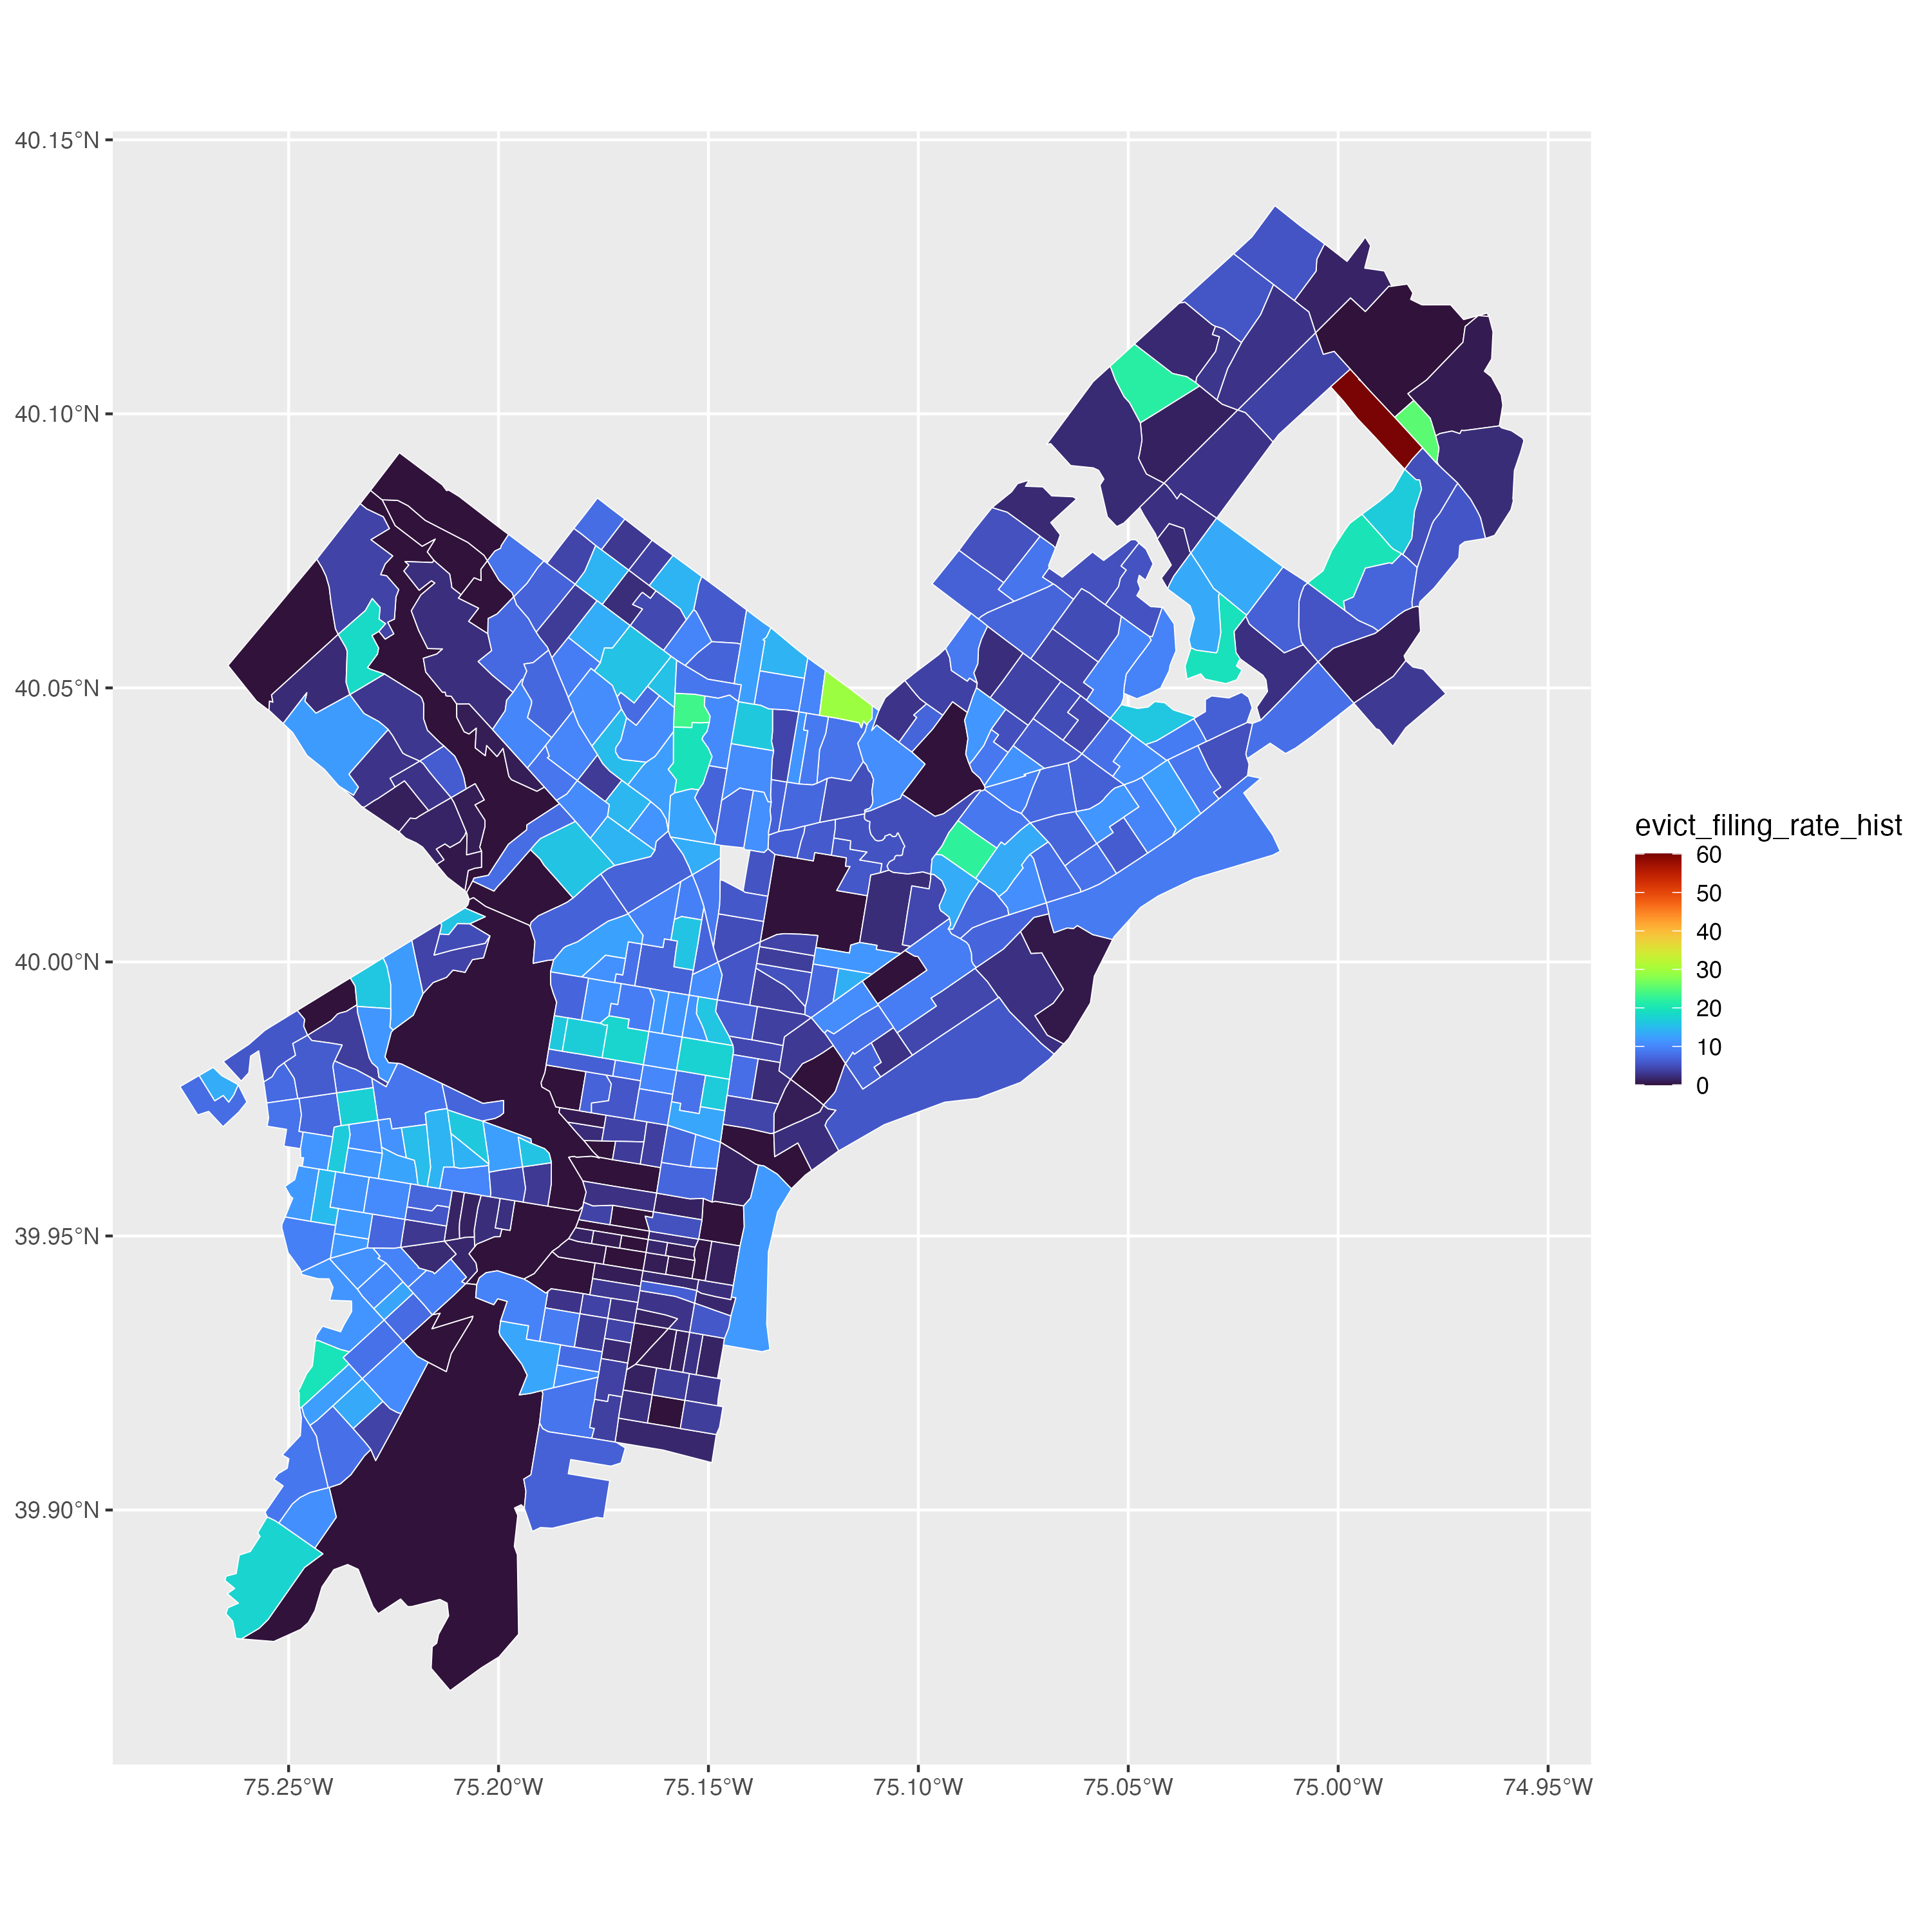
\includegraphics[width=0.6\linewidth]{figs/evict_filing_rate_hist.png}
    \caption{Evictions in Philadelphia (2019)}
    \label{fig:philly-map}
\end{figure}

Secondly, I show that, when looking across properties, evictions are concentrated in a hand full of buildings. To show this, I merged the eviction data, which contain the defendant's address, with the rental registry and the parcel data in Philadelphia. This lets me know which properties are rental units in a given year, as well as the number of rental units that are in each property. Doing this allows me to plot the CDF of eviction filings alongside the CDF of rental units. \\

As \ref{fig:philly-evict-parcel} shows, the vast majority of rental units do not file an eviction in a typical year. Of the properties that do file an eviction, most file only one. There are, however, a handful of properties, comprising less than 1\% of the overall rental housing stock that file over 25\% of evictions. 

\begin{figure}[htbp]
    \centering
    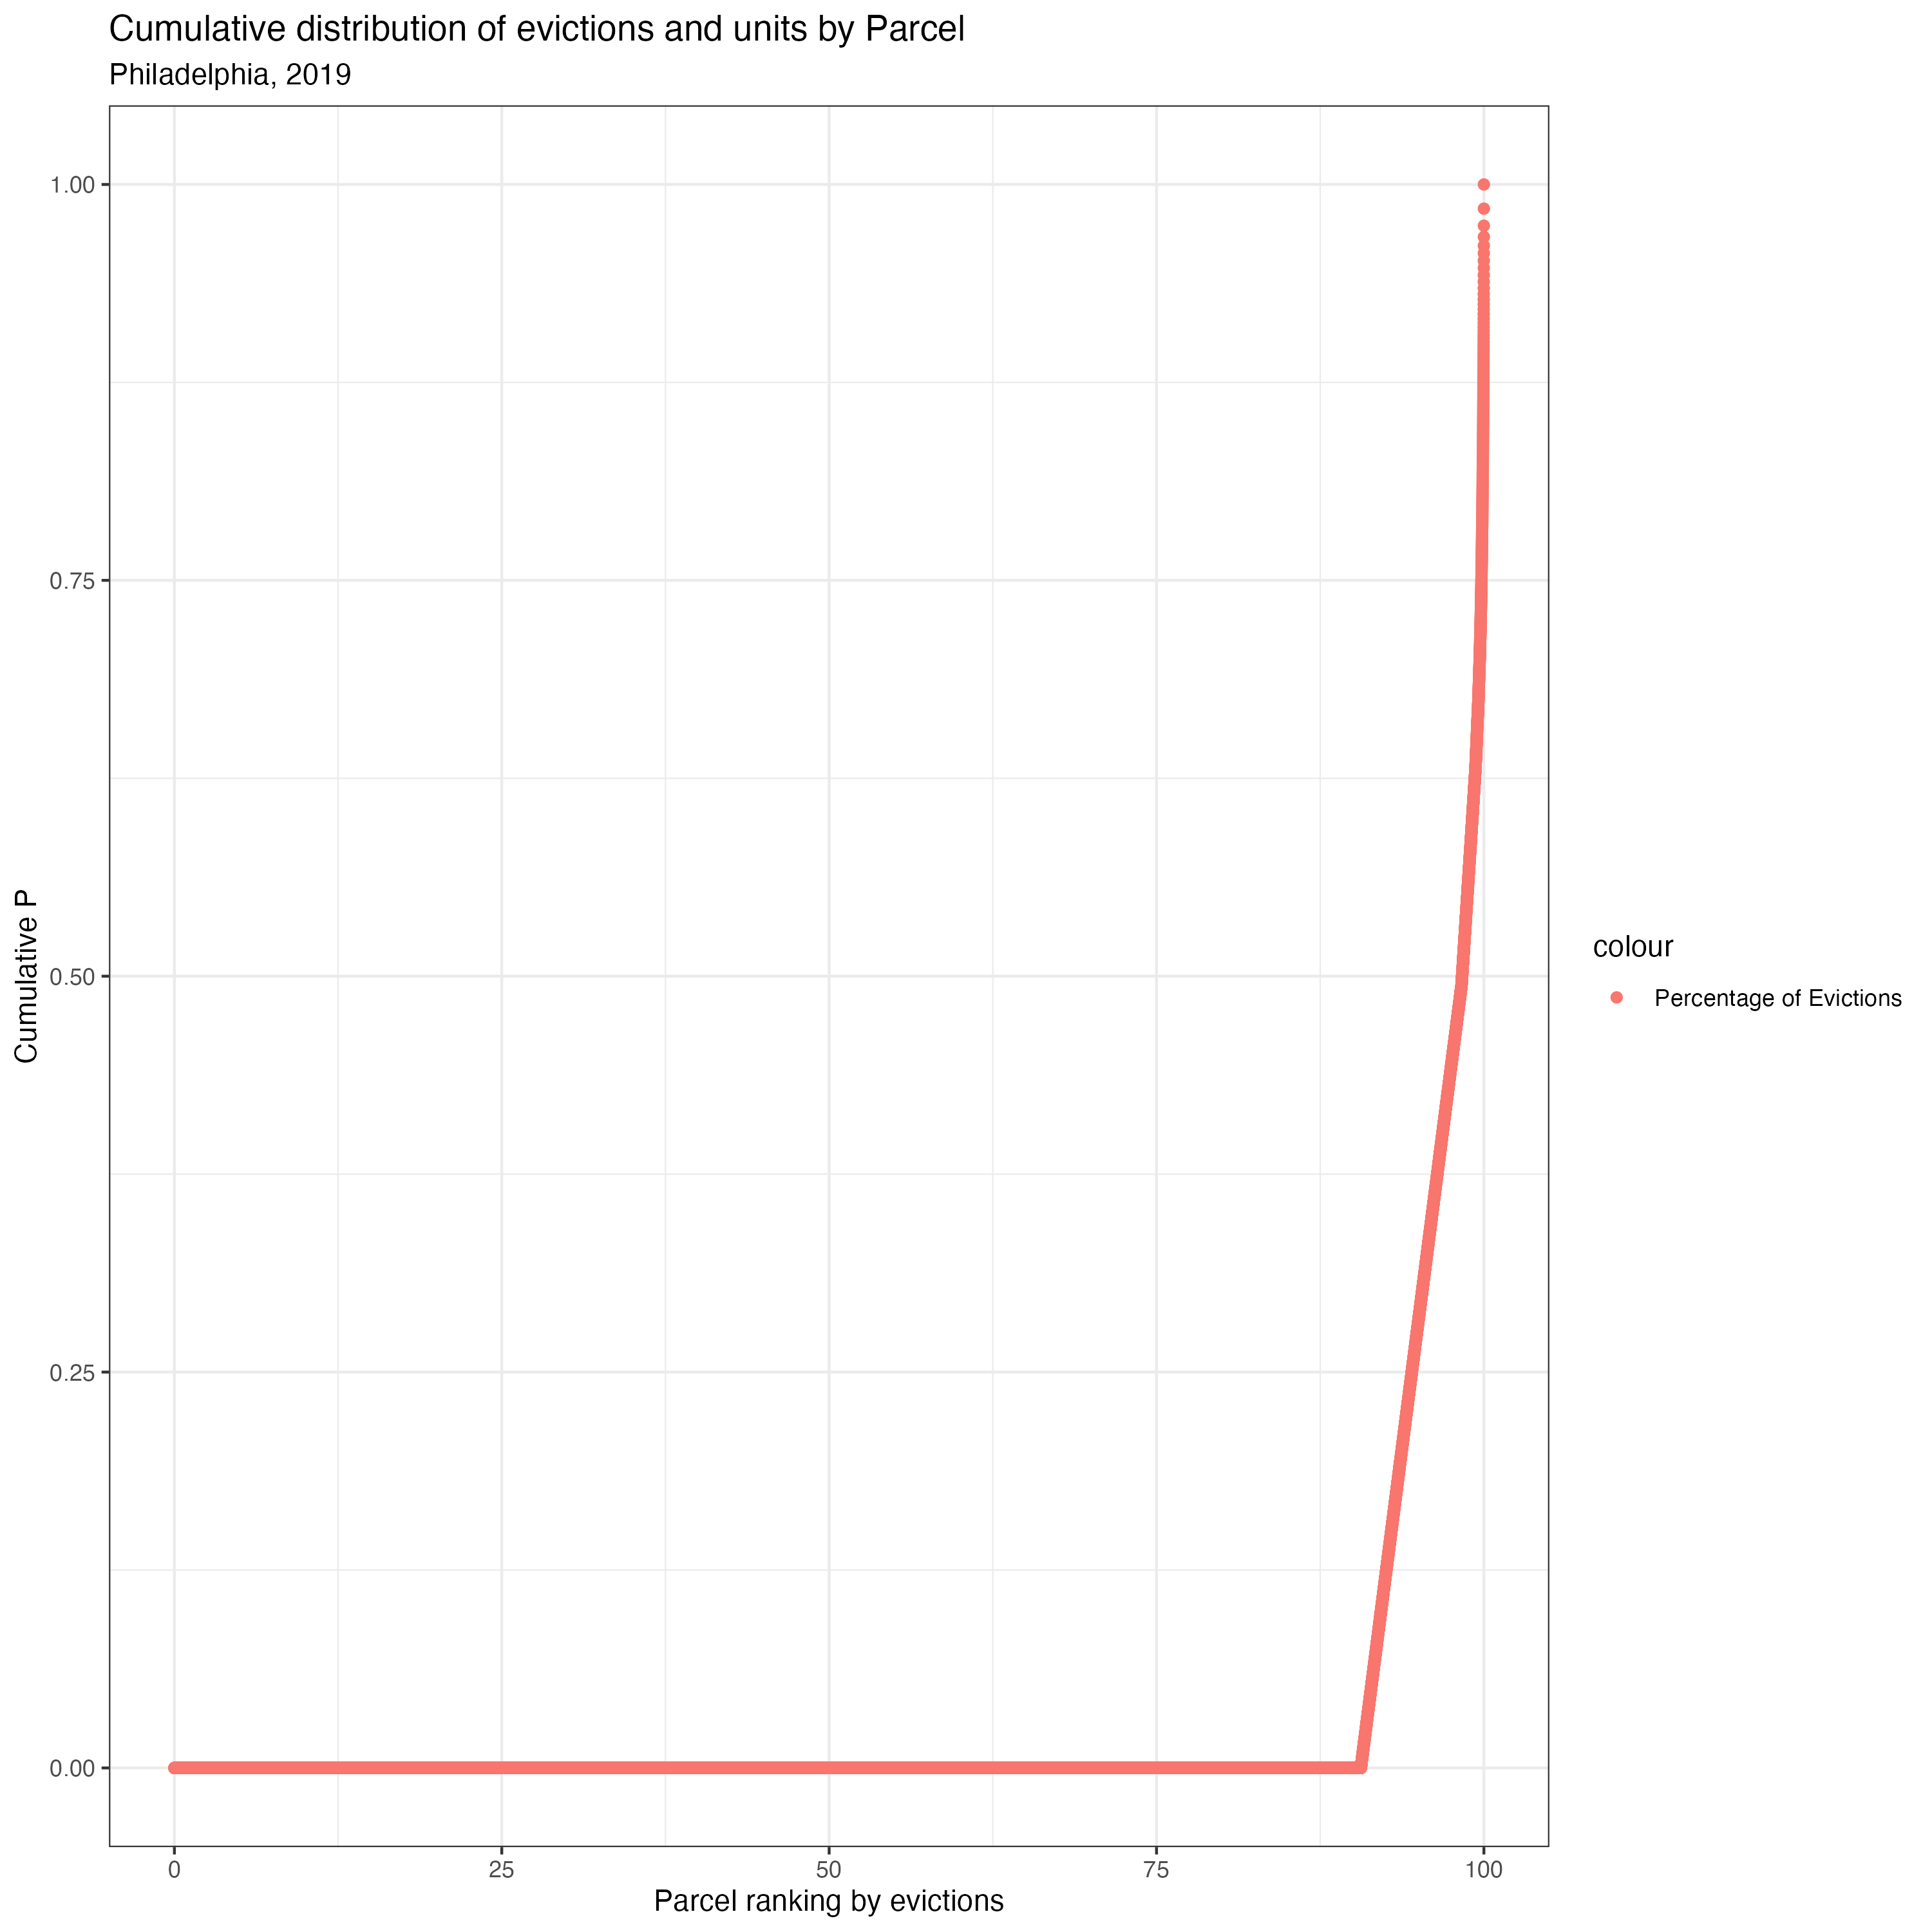
\includegraphics[width=0.6\linewidth]{figs/cumulative_evict_dist_parcels.png}
    \caption{Evictions in Philadelphia}
    \label{fig:philly-evict-parcel}
\end{figure}

Third, in table \ref{tab:philly-rent}

\begin{table}[htbp]
    \begin{longtable}{l|rrrr}
\caption*{
{\large Summary Statistics on Philadelphia Rent Prices} \\ 
{\small 2010-2019}
} \\ 
\toprule
\multicolumn{1}{l}{} & \multicolumn{2}{c}{Rent} & \multicolumn{2}{c}{Number of Evictions} \\ 
\cmidrule(lr){2-3} \cmidrule(lr){4-5}
\multicolumn{1}{l}{} & non-Top Evictor & Top Evictor & non-Top Evictor & Top Evictor \\ 
\midrule\addlinespace[2.5pt]
2010 & $675$ & $634$ & 14649 & 6674 \\ 
2011 & $685$ & $654$ & 14979 & 6498 \\ 
2012 & $700$ & $654$ & 15271 & 6642 \\ 
2013 & $700$ & $675$ & 15366 & 6064 \\ 
2014 & $725$ & $707$ & 15645 & 6257 \\ 
2015 & $750$ & $725$ & 14395 & 5891 \\ 
2016 & $750$ & $800$ & 14994 & 5622 \\ 
2017 & $775$ & $825$ & 14627 & 5748 \\ 
2018 & $800$ & $970$ & 11987 & 3735 \\ 
2019 & $850$ & $1,050$ & 11763 & 3473 \\ 
\bottomrule
\end{longtable}


    \caption{Philadelphia Rent}
    \label{tab:philly-rent}
\end{table}


\subsection{Evictions in Philadelphia over time}

\begin{figure}[htbp]
    \centering
    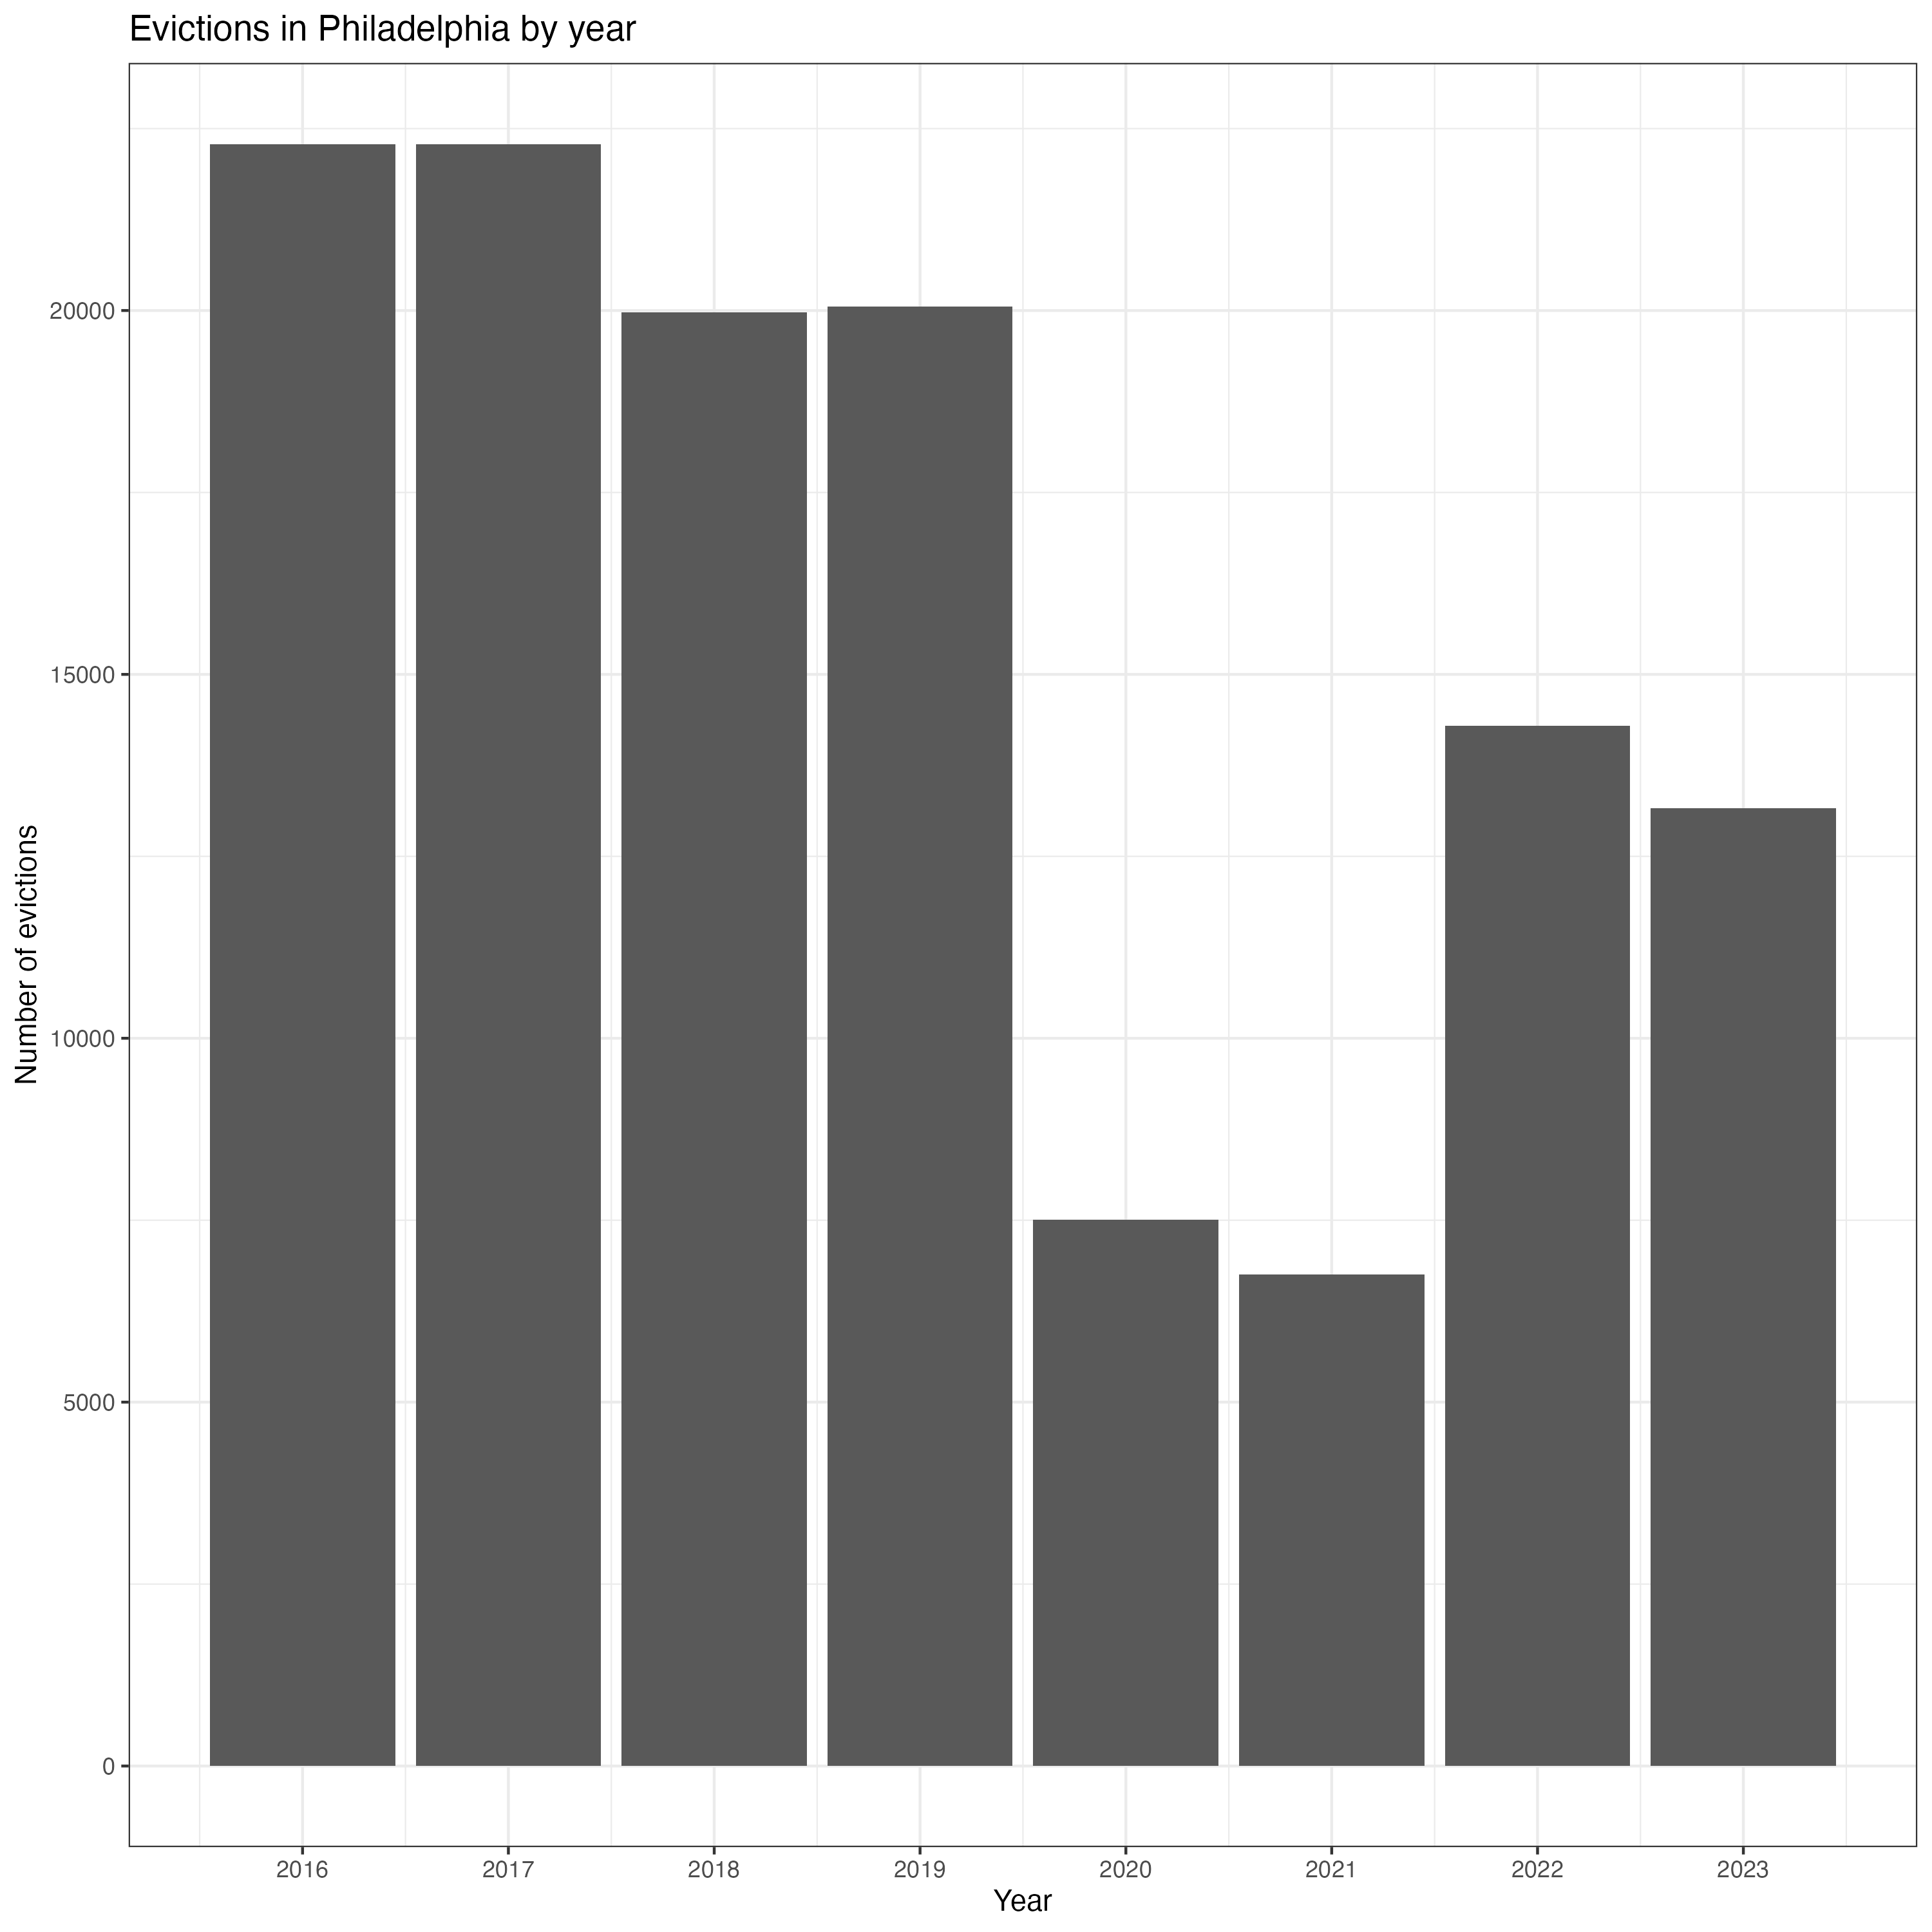
\includegraphics[width=0.6\linewidth]{figs/evict_by_year.png}
    \caption{Evictions in Philadelphia}
    \label{fig:philly-year}
\end{figure}



\subsection{Rent Prices in Philadelphia}

\section{Research Questions and Empirical Specifications}

\subsection{Descriptive Evidence on Pricing and Eviction Filing Behavior}

The first set of findings I'd like to document are related to landlord pricing and filing behavior. Specifically:

\begin{itemize}
    \item Do high evicting landlords charge higher rents relative to similar properties?
    \item Are thresholds (back rent required for eviction filing to occur) for high evicting landlords different from those for lower evicting landlords. 
    \item Building on Alison Lodermeier's job market paper, a natural question would be whether high evicting landlords are more likely to statistically or tasted-basely discriminate against their tenants, relative to lower evicting landlords 
    \item Are high evicting landlords also likely to be serial evictors -- meaning they use eviction both as a debt collection tool and as one to remove tenants.
\end{itemize} \\

As these are all descriptive findings, I think the identification is relatively straightforward. The main consideration will be what "similar property" means -- I think for now it will be defined geographically, assuming there aren't large rental gradients within the same neighborhood.


\subsection{Sorting into high evicting properties}
A key question with the low income rental market is to what extent these high evicting properties are providing "housing of last resort" to those with previous eviction or conviction histories, or whether these buildings are high evicting due to their landlord's business model, even conditional on tenant selection. Given the empirical evidence of the negative consequences of eviction, and the distinct possibility that these properties could be providing housing to a segment of the market that might otherwise be homeless, this is an important question to get correct. \\

As a first step, I want to know whether the tenants at these high evicting properties different across observable characteristics (race, prior eviction history, credit score, etc.) than those who sort into lower evicting properties. My expectation is that these tenants are more risk, however, the precise magnitudes would be an important empirical finding. One question I would like to answer, but which I'm struggling with how to do, would be to estimate the effect on <outcomes> of ending up in one of these buildings. \\


\subsection{Landlord responses to changes in tenant protections}

The next set of questions pertain to how landlords respond to changes in their ability to evict their tenants. As documented by cite, during the eviction moratoria, landlords increased their discrimination against Black and Hispanic tenants, suggesting that landlords do respond to changes in rental market institutions. My analysis would build on this and ask the following questions:\\

As a result of both the eviction moratoria and Philadelphia's eviction diversion program:\\


\begin{itemize}
    \item Do landlords pass on the higher cost of evictions to tenants?
    \item Do landlords exit the market following a change in the legal climate?
    \item Do landlords change their behavior on other margins (rent to different kinds of tenants, make upgrades/downgrades to the property, etc.)
\end{itemize} \\

The key identification issue will be defining an appropriate control group, both because the eviction moratoria was temporary and because under both the moratoria and the eviction diversion program, the whole city is being treated. One option would be to try and define a synthetic Philadelphia, although this is complicated because other cities do not have the same quality of rental data. Another option would be to try a shift share approach where landlords shares are their pre-treatment reliance on eviction and the shock is either the COVID moratoria and/or the eviction diversion program. \\

Another interesting angle is heterogeneity by landlord type. From interviews, landlords place a high value on the option of evicting a tenant (and claim there's a high compliance cost of landlord tenant laws), but empirically, relatively few landlords file an eviction in a given year-- in most cities I've checked, it's around half of apartment complexes with greater than ten units will file an eviction, but there's only 6 filings per every hundred units. To me, this suggests that there might be quite a lot of wiggle room to reduce evictions without doing much to change landlord behavior.



\subsection{Welfare Analysis}

The big hope of the paper would be to get the "correct" model of the low income rental market. In addition to the pass through analysis, analysis of exit decisions, and other margins of landlord adjustment, I'd like to put a dollar sign on the option value of being able to evict (with some probability). If you add that, plus rent increases (if they exist), you'd get a "cost" of the program. To my knowledge, no one has put out the "social cost of an eviction" number, but that would be the ideal to benchmark against. \\

Big picture, "what's the correct way to regulate slum lords" is a question that has a lot of relevance, both in contemporary America, but also globally. There are some interesting historical parallels between New York City's tenement regulations, which to my knowledge were broadly successful, and New York City's 1955 ban on new single room occupancy hotels, which is generally attributed to a rise in homelessness.



\end{document}